%%%%%%%%%%%%%%%%%%%%%%%%%%%%%%%%%%%
%       code starts here
%%%%%%%%%%%%%%%%%%%%%%%%%%%%%%%%%%%
\documentclass[12pt]{article}
%\pagestyle{empty}
%headings, myheadings, plain, empty
\usepackage{amsmath}
\usepackage{amstext}
\usepackage{amssymb}
\usepackage{graphicx}
\usepackage{amsfonts}
\usepackage{amsthm}
\usepackage{geometry}
\usepackage{booktabs}
\usepackage{float}
\usepackage{fixmath}
\usepackage{hyperref}
\usepackage{tabularx,ragged2e,booktabs,caption}
%\usepackage[framed,numbered]{mcode}

\geometry{hmargin = 1in, vmargin=1in}
\setlength{\parskip}{1.0ex}
\setlength{\parindent}{4mm}

\columnseprule 1pt

\newcommand\R{\mathbb{R}}
\newcommand\N{\mathbb{N}}
\newcommand\C{\mathbb{C}}
\newcommand\Z{\mathbb{Z}}
\newcommand\T{\mathcal{T}}
\newcommand\X{\mathcal{X}}
\newcommand\F{\mathcal{F}}
\newcommand\Oh{\mathcal{O}}

\newcommand\beq{\begin{eqnarray*}}
\newcommand\eeq{\end{eqnarray*}}
\newcommand\clb{\begin{flushright}$\clubsuit$\end{flushright}}
\newcommand\str{\begin{flushright}$\bigstar$\end{flushright}}
\newcommand\spd{\begin{flushright}$\spadesuit$\end{flushright}}
\newcommand\dmd{\begin{flushright}$\diamondsuit$\end{flushright}}
\newcommand\limplies{\Longleftarrow}

\theoremstyle{plain} %italic
\newtheorem{claim}{Claim}
\newtheorem{theorem}{Theorem}
\newtheorem{prop}{Proposition}

\theoremstyle{definition} %roman
\newtheorem{defn}{Definition}
\newtheorem{prob}{Problem}
\newtheorem*{soln}{Solution}
\newtheorem*{pf}{Proof}
\newtheorem{example}{Example}

\theoremstyle{remark} %roman
\newtheorem{rmk}{Remark}
\newtheorem{note}{Note}
\newtheorem{case}{Case}

\begin{document}
\title{Udacity Machine Learning Nanodegree: \\ Sberbank Housing Price Prediction}
\author{Joe Dinius \\ Capstone Project}
%\address{University of Arizona}
%\email{jdinius@math.arizona.edu}
\date{\today}
\maketitle
\section{Introduction}
\subsection*{Project Overview}
\indent \par The first project for this course was predicting housing prices in Boston based on a simple feature set.  This project will build on some of the intuition that was built while completing that project.

\par The website \href{https://www.kaggle.com}{Kaggle} is currently hosting a competition that requires implementation of regression techniques like those used in the Boston housing prediction project.  Sberbank, the Russian bank, along with Kaggle, is hosting a competition to predict Russian housing prices based on a dataset rich in features.  According to the \href{https://www.kaggle.com/c/sberbank-russian-housing-market}{project introduction page}, the Russian housing market is relatively stable when compared to the more volatile Russian economy as a whole.  Having an accurate predictor would help to assure both investors and prospective property owners that they are making wise choices in how they invest in Russian real estate despite other potentially worrying economic indicators.

\subsection*{Problem Statement}
\indent \par Kaggle has provided a full dataset broken into training and test datasets.  This dataset provides features from which a regression model will be used to predict housing prices based on the values of these features.  A standard regression technique such as the one used for the Boston housing prediction project will most likely not perform well on the larger, more nuanced feature set that will be used for this project.  A more flexible learner is needed.  The package \href{http://xgboost.readthedocs.io/en/latest}{\textbf{XGBoost}} is a fully integrated, flexible framework for performing gradient boosting regression using multiple simple learners, such as decision trees.  The combination of simple learners into a more complex single learner has been very successful in both supervised machine learning problems.  The reason \textbf{XGBoost} in particular is chosen as the starting point is its \href{https://github.com/dmlc/xgboost/tree/master/demo#machine-learning-challenge-winning-solutions}{success} in previous machine learning competitions.

\par The solution to this project has two parts:  (1) tuning a regressor to minimize the prediction error of housing prices on validation data extracted from the training set provided and (2) predicting prices on the Kaggle-provided test set using regressors developed during the tuning process.  The prediction data on the test set will be submitted to Kaggle for internal computation of a public score.  The public score is used to rank solutions and will be used as a sanity check on the algorithm's performance.  The desired public score is as close to 0 as possible; lower scores are better than higher ones.

\subsection*{Metrics}
\indent \par The primary metric here, as in most regression problems, is error on a test set with known output.  The error metric used for optimization is the negative of the \href{https://en.wikipedia.org/wiki/Mean_squared_error}{mean squared error}
\beq
S_{\text{residual}} \equiv \text{mean squared error} = \sum_i \bigl ( y_{\text{actual},i} - y_{\text{predicted},i} \bigr )^2,
\eeq
where $y_*$ represents the target variable of the regression.  This provides a strong estimate of how well matched predictions are to actual observations.  Since the error is averaged over all elements of a dataset (training or validation), this provides a quantitative assessment of model quality. The negative is chosen on account of the \textbf{sklearn} protocol where the negative is used in a maximization scheme; that is, minimizing error is equivalent to maximizing the negative of that same error.  

\par Another metric will be used as well.  In cross-validation efforts, the model's predictive power will be evaluated using the $R^2$ score, also known as the \href{http://stattrek.com/statistics/dictionary.aspx?definition=coefficient_of_determination}{coefficient of determination}.  The mathematical formula for the $R^2$ score is
\beq
S_{\text{total}} &=& \sum_i \bigl ( y_{\text{actual},i} - \bar y \bigr )^2 \\
R^2 &\equiv& 1 - \frac{S_{\text{residual}}}{S_{\text{total}}},
\eeq
where 
\beq
\bar y = \frac{1}{n} \sum_{i=1}^n y_{\text{actual},i}
\eeq
is the mean of the observed test target variable data.  A score of 1 means that the model perfectly predicts the output for each given input, while a score of -1 means that the model is completely unable to predict output based on the given input.  The goal is an $R^2$ score that is positive and as close to 1 as possible.

\section{Analysis}

\indent \par As a starting point, \href{https://www.kaggle.com/captcalculator/a-very-extensive-sberbank-exploratory-analysis}{this} was used for reference.

\subsection*{Data Exploration}
\indent \par The dataset provided is captured in three csv files: \href{./data/train.csv}{train.csv}, \href{./data/test.csv}{test.csv}, and \href{./data/macro.csv}{macro.csv}.  
The columnar data of the csv files are described in \href{./data/data_dictionary.txt}{data\_dictionary.txt}, please see this file for description of the individual features.  The columns in train.csv and test.csv represent data about the properties themselves, along with timestamps; data such as square footage (size), number of rooms, and build year.  Extrinsic properties, such as proximity to entertainment and cultural attractions, are also included in these csv files.  The column \textbf{price\_doc} denotes the sale prices of the properties, and is the target variable for the regression analysis.  Data within macro.csv, as the name would indicate, presents broad macroeconomic indicators along with timestamps.  These data include gross domestic product, currency exchange rates, and mortgage rates.

An initial sense of how the sales price, \textbf{price\_doc}, is distributed is a good place to start the analysis.  This can be accomplished with a simple histogram (see Figure \ref{fig:one}):
\begin{figure}[h!]
\begin{center}
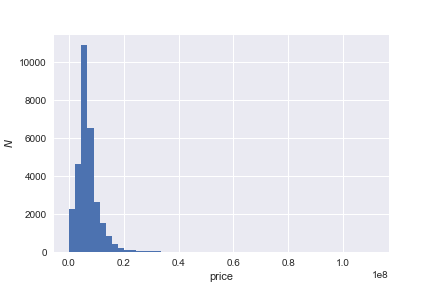
\includegraphics[width=12cm]{./output_images/price_doc_hist.png}
\caption{Histogram of sales price, $p$}
\label{fig:one}
\end{center}
\end{figure}

The data appears to be positive-definite and may well be lognormal distributed.  In regression analyses, when some variables appear to be lognormal, \href{https://www.analyticsvidhya.com/blog/2016/01/guide-data-exploration/#four}{taking the log can reduce variation caused by outliers in the original distribution}.  The histogram is replotted after adding 1 (to avoid divergence of the logarithm function) and then taking the natural logarithm (see Figure \ref{fig:two}):

\begin{figure}[h!]
\begin{center}
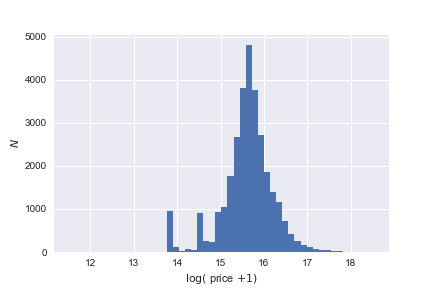
\includegraphics[width=12cm]{./output_images/price_doc_log_hist.png}
\caption{Histogram of logged sales price, $\log(1+p)$}
\label{fig:two}
\end{center}
\end{figure}

The resulting histogram above seems to indicate a mostly normal distribution; there is apparent symmetry about a central value between 15 and 16.  Going forward, the transformed price variable will be used as the new target variable for the regression analysis. This should enable the model to be more robust to variation caused by extrema in the price data.

Next, explore the top-level statistics of the intrinsic properties of the real estate:
\begin{center}
\captionof{table}{Top-level statistics of intrinsic properties}
\begin{tabular}{c | c | c | c }
\hline
Property (metric) & mean & median & standard deviation \\ \hline
\textbf{full\_sq} & 53.70 & 50.41 &  20.10 \\ \hline
\textbf{life\_sq} & 32.66 & 30.40 &  22.74 \\ \hline
\textbf{kitch\_sq} & 6.94 & 7.00 &  25.58 \\ \hline
\textbf{num\_rooms} & 1.88 & 2.00 &  0.84 \\ \hline
\end{tabular}
\label{tbl:one}
\end{center}

Table \ref{tbl:one} variables show close connection between the mean and median values.  What is surprising is the large variation in kitchen size.  In fact, there is larger variance in this feature than in the full property size!

One might like to get a better idea of how some of these data are distributed.  One such data trend that would of interest would be price versus the year the property was built (see Figure \ref{fig:three}).

\begin{figure}[h!]
\begin{center}
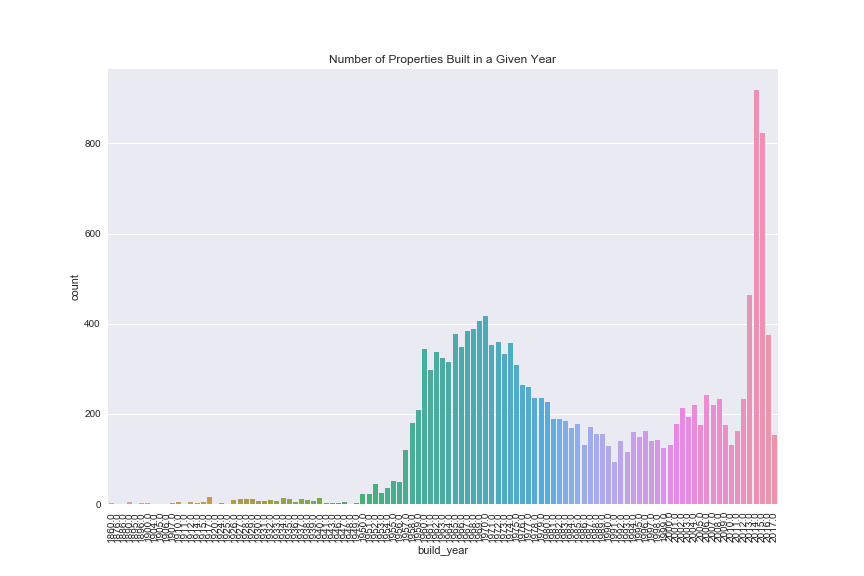
\includegraphics[width=18cm,height=9cm]{./output_images/properties_year.png}
\caption{Frequency of properties built for a given year}
\label{fig:three}
\end{center}
\end{figure}

From the plot Figure \ref{fig:three}, it is clear that a majority of properties sold have been built more recently (\textbf{build\_year} $> 2013$).  However, it is interesting to note the large amount of construction in the late 1950's and early 1960's, and the subsequent dip in housing production culminating in a minimum in 1991, near when the Soviet Union collapsed.  This is purely speculation at this point, and doesn't really hold much weight in the analysis that follows.  However, it is not inconceivable that such a trend would positively correlate with macroeconomic indicators, such as GDP.  Data related to that reported in Figure \ref{fig:three} would be the mean sale price versus the build year.  Figure \ref{fig:four} shows this data, along with a third order regression with the 95\% confidence interval. 

\begin{figure}[h!]
\begin{center}
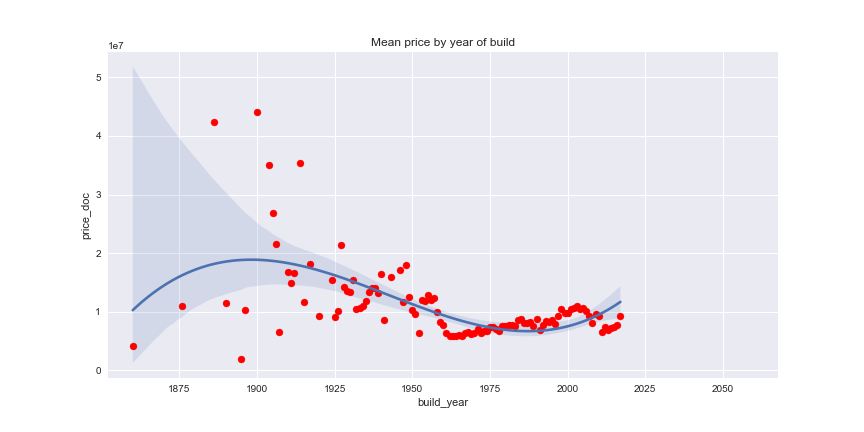
\includegraphics[width=12cm]{./output_images/mean_price_year.png}
\caption{Mean price, plus confidence interval, of price for a given year}
\label{fig:four}
\end{center}
\end{figure}

\par Figure \ref{fig:four} demonstrates a more easily predictable trend for properties built more recently (\textbf{build\_year} $> \approx 1945$).  The inherent accuracy of such predictions can be seen from the tight variance bounds around the simple regression plotted alongside the raw data.  The reduction in variability could be a result of more uniformity in housing projects during the Communist years, or for some other reasons.  Again, this is merely an observation and doesn't impact the analysis that follows.

\par Another nice plot would be something that would show price as a function of the condition of the property.  A box-plot would work, and the \textbf{state} variable encodes the conditions of the properties.

\begin{figure}[h!]
\begin{center}
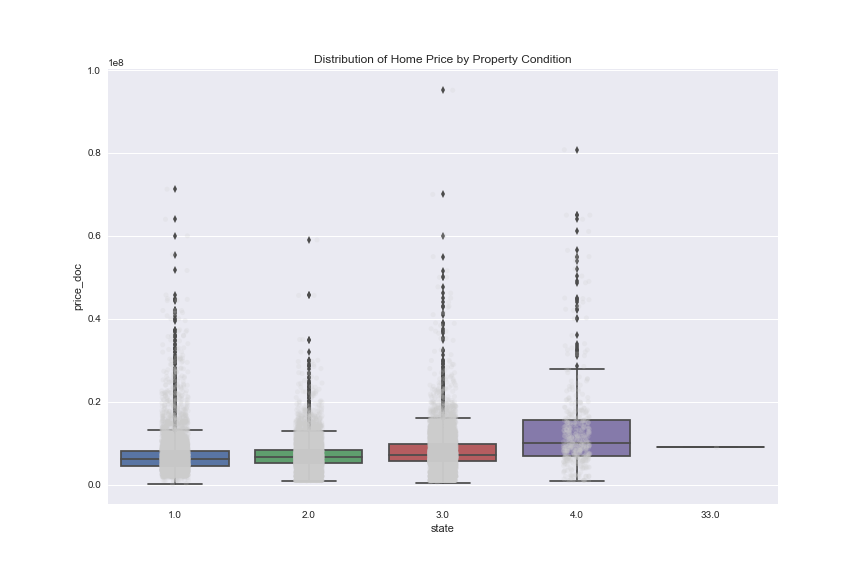
\includegraphics[width=8cm]{./output_images/state_box_plot.png}
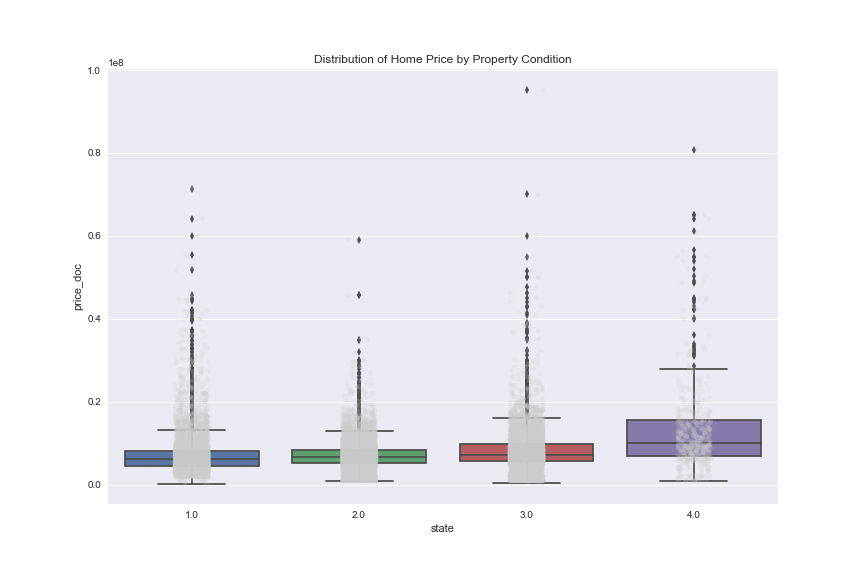
\includegraphics[width=8cm]{./output_images/state_box_plot_fixed.png}
\caption{Box plots of condition versus price.  Left: erroneous state 33, Right: corrected}
\label{fig:five}
\end{center}
\end{figure}

Figure \ref{fig:five} demonstrates a few interesting points.  The first is a data quality issue; namely, what does \textbf{state} $= 33$ mean?  After looking into the dataset itself and at forums on the Kaggle competition page, this seems to be an invalid state.  Given the frequency of occurrence and the easy-to-do data entry error of entering multiple of the same number in the same data cell, it seems the entry was made in error and the appropriate state in these instances should be \textbf{state} $= 3$.  The original dataset can now be updated in light of this new information and the data can be replotted (see right side of Figure \ref{fig:five}).

\par The trends observed tend to make sense.  Price increases with increasing condition, or quality, of the property.  Also, properties with the lowest and highest conditions occur less frequently than those properties in just so-so condition.  Properties in the highest condition tend to have higher variability in price.  This could be as a result of high quality properties having variability in size, number of rooms, and other intrinsic properties.  There may be other trends as well; namely, extrinsic properties  (e.g. proximity to shopping, grocery stores, schools, etc...) may have an impact on price.

Before moving on with the data exploration, another irregularity is present in the dataset.  This was highlighted in the Kaggle forums for the competition and is pretty simple to fix.  Some of the \textbf{build\_year} data has been incorrectly entered and just needs to be updated with a valid date.  Through inspection of the raw data, it's clear that much data is missing (indicated by \textbf{NA} in the cells).  The most frequently missing data, along with the frequency missing, is plotted in Figure \ref{fig:six}.

\begin{figure}[h!]
\begin{center}
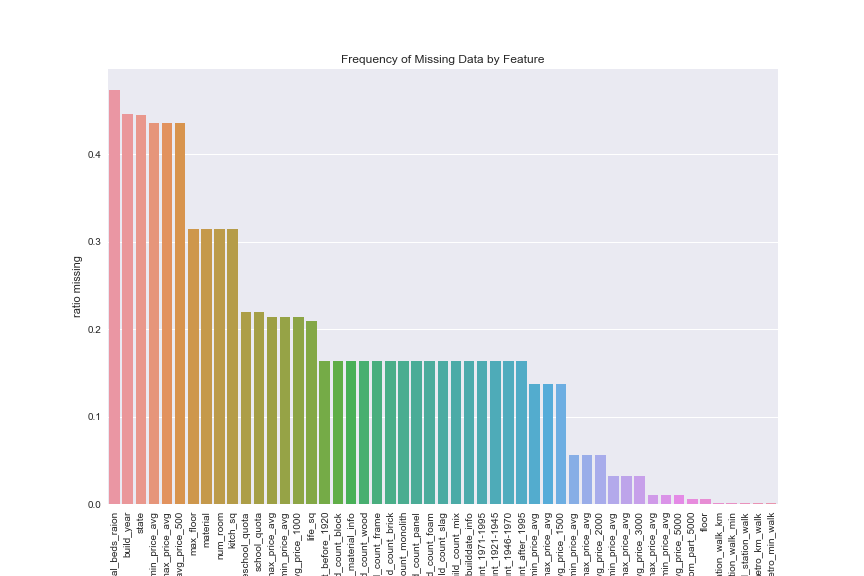
\includegraphics[width=18cm,height=9cm]{./output_images/missing_frequency.png}
\caption{Frequency of missing data}
\label{fig:six}
\end{center}
\end{figure}

(It should be mentioned here that "raion" indicates an area around the property, kind of like a region would be in English-speaking nations.)

For some of the data, it is not particularly surprising that values are missing.  Something like the number of hospital beds in a region may be a difficult number to come by in a real estate search.  However, it is worth noting that a number of common property features are missing with surprisingly large frequency.  Factors such as \textbf{state}, the condition of the property should definitely be recorded as part of any real estate transaction.  If it were simply missing because there is no property state (i.e. the property is a vacant lot), then this should be encoded as a separate class within the data.

\subsection*{Exploratory Visualization}
\indent \par A good first thing to consider is the importance of individual features. Arguably, the best starting point is how price relates to intrinsic features of properties.  Heatmaps show how correlated one variable is to others and are great indicators of interrelatedness within data.  The heatmap in Figure \ref{fig:seven} shows interrelatedness between intrinsic data of properties.

\begin{figure}[h!]
\begin{center}
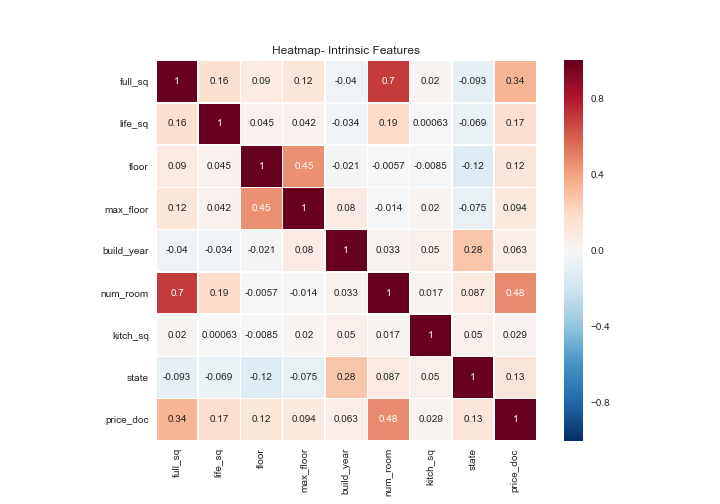
\includegraphics[width=15cm]{./output_images/intrinsic_heatmap.png}
\caption{Intrinsic features heatmap}
\label{fig:seven}
\end{center}
\end{figure}

\par The biggest correlations to price are seen in \textbf{full\_sq} and \textbf{num\_room}.  This makes sense; increasing square footage and number of rooms should increase the sale price.  Also, not surprisingly, the state and floor of the property (in the case of apartments) are also positively correlated with sale price.

\par In the heatmap presented in Figure \ref{fig:seven}, trends between intrinsic properties were made clear.  These data showed a somewhat predictable trend: more square footage tended to mean a higher sales price.  Less clear, however, is the correlation between extrinsic properties and price.  Again, a heatmap will be illuminating here.  Look at some of the more broad features, features pertaining to local population.

\begin{figure}[h!]
\begin{center}
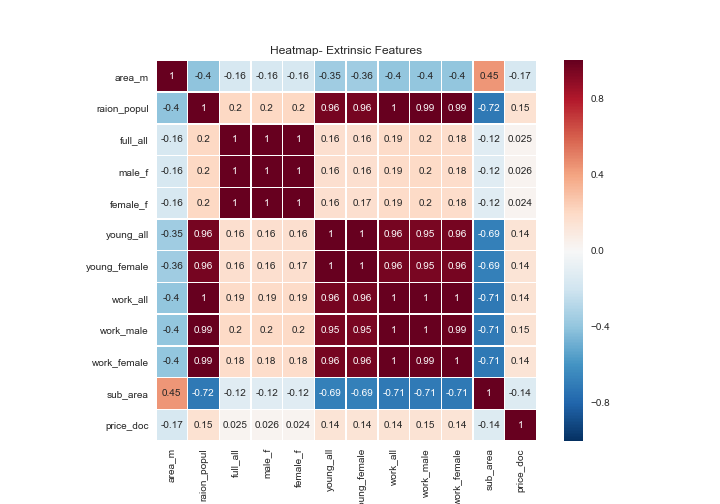
\includegraphics[width=15cm]{./output_images/extrinsic_heatmap.png}
\caption{Extrinsic features heatmap}
\label{fig:eight}
\end{center}
\end{figure}

The variables shown in Figure \ref{fig:eight} are mostly concerned with aspects of the regions themselves.  These data include region population, along with a breakdown on working age (\textbf{work\_*}) and youth (\textbf{young\_*}) populations.  Not surprisingly, there is moderate correlation between the region name and the area of that region.  This isn't, strictly-speaking, important to the analysis; it's just an observation.  Also, the population characteristics are highly correlated to one another; that is, the working age male population of an area (\textbf{work\_male}) is highly correlated with the working age female population (\textbf{work\_female}) of that same area.

There doesn't appear to be a strong correlation to any of these variables with the sales price.  Maybe other extrinsic features will show more correlation.  There are so many of these features, and they can be broken down into categories:  school, entertainment, and infrastructure.

Consider school characteristics first (see Figure \ref{fig:nine}):

\begin{figure}[h!]
\begin{center}
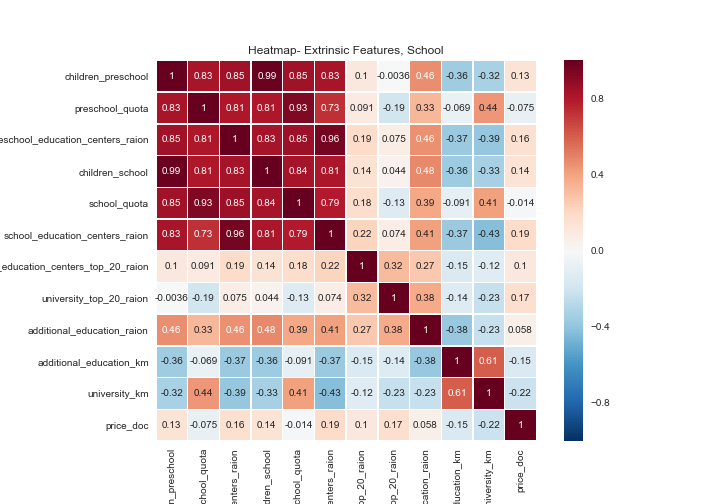
\includegraphics[width=15cm]{./output_images/school_heatmap.png}
\caption{School feature heatmap}
\label{fig:nine}
\end{center}
\end{figure}

The population of school-age children shows a moderate correlation with sales price, as expected. The degree of correlation is less than expected given naive assumptions about proximity to schools being a prime factor in real estate in the United States.  Of note, as well, is the negative correlation of sales prices with distance to universities.  It makes sense that, the farther one is from a university, the lower the sales price.  This trend exists in the US as well, since real estate close to universities is very desirable, and fetches a larger sales price typically.

Next, consider entertainment features (see Figure \ref{fig:ten}):

\begin{figure}[h!]
\begin{center}
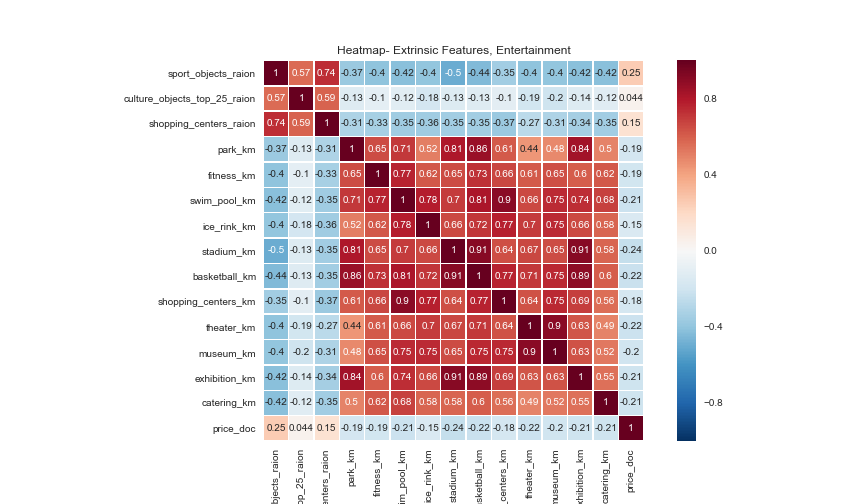
\includegraphics[width=15cm]{./output_images/entertainment_heatmap.png}
\caption{Entertainment feature heatmap}
\label{fig:ten}
\end{center}
\end{figure}

The data above again makes sense in the aggregate: the farther a property is from recreational attractions, like shopping centers or museums, the lower the sales price.  Put another way, real estate near cultural and recreational attractions is more desirable and is typically more valuable.

Finally, infrastructure features are considered (see Figure \ref{fig:eleven}):

\begin{figure}[h!]
\begin{center}
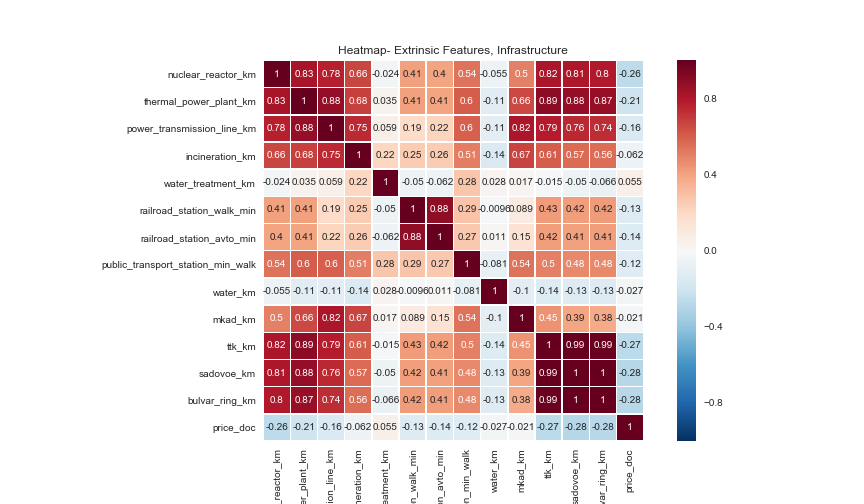
\includegraphics[width=15cm]{./output_images/infrastructure_heatmap.png}
\caption{Infrastructure feature heatmap}
\label{fig:eleven}
\end{center}
\end{figure}

The data above is surprising.  Naively, one would assume that being closer to power generation stations would be undesirable and would show positive correlation with price.  However, the data indicates otherwise.  Other data, like correlation of price with distance to public transportation, makes sense in the context provided.

Next, consider correlation between price and macroeconomic indicators  (see Figure \ref{fig:twelve}):

\begin{figure}[h!]
\begin{center}
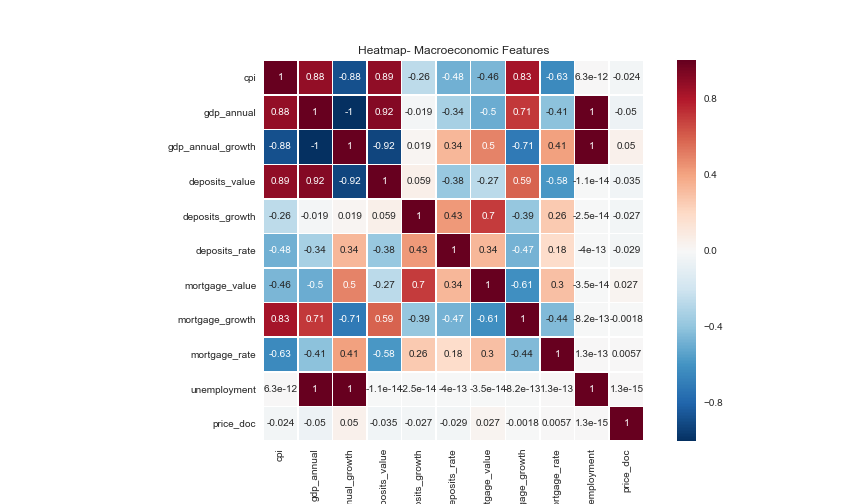
\includegraphics[width=15cm]{./output_images/macro_heatmap.png}
\caption{Macroeconomic feature heatmap}
\label{fig:twelve}
\end{center}
\end{figure}

This data is pretty interesting.  As expected, intrinsic and extrinsic properties of the real estate are much more correlated to sales price than broader macroeconomic features.  This is exactly as one would expect.  It is surprising, though, that mortgage properties aren't more positively correlated with price.  It would seem that lower mortgage rates might entice more buyers, and with more buyers, one might expect higher prices.  However, the data shows almost no correlation to price.  It is also interesting that prices aren't more negatively correlated with unemployment.  Again, naively, it would seem that higher unemployment would mean lower prices on real estate transactions.

\subsection*{Algorithms and Techniques}
\indent \par As mentioned previously, \textbf{XGBoost}, along with the \textbf{sklearn} wrapper \textbf{XGBRegressor}, will be used for performing the regression analysis.  

\par \textbf{XGBoost} uses tree ensembles: sets of classification and regression trees (CART).  A CART is different from a decision tree in that decision trees provide only decision values, whereas CARTs provide real scores for each leaf.  The tree ensemble then uses the sum of prediction of a target variable for multiple trees.  \textbf{XGBoost} utilizes additive training (also known as boosting), where each new tree is added with full knowledge of what has already been learned.  Put another way, the updated model at each training round incorporates the model learned from the previous state.  To this previous model is added a new tree which decreases training loss and minimizes complexity of model; the complexity is controlled via regularization parameters that are hyperparameters of the model.  See \href{http://xgboost.readthedocs.io/en/latest/model.html}{this resource} for more details.

\par This package was chosen because of its success in machine learning competitions of various scales.  The use of boosted trees will allow for a model that requires minimal feature engineering (see \href{https://www.kaggle.com/c/allstate-claims-severity/discussion/24500}{this}); all that needs to be done is hyperparameter tuning.  The package \textbf{sklearn} has two very nice optimization frameworks for estimator tuning: \textbf{RandomizedSearchCV} and \textbf{GridSearchCV}.  \textbf{RandomizedSearchCV} allows for sampling the parameter space by random draws from probability distributions.  The choice of distribution depends upon the parameter being tuned, however the uniform distribution is a great choice; this is because it allows for sampling of a spatial structure where each point has equal probability.  The equal probability is desirable since, a priori, there are minimal assumptions made about model performance as a function of the hyperparameters.

As with all regression techniques, a model is developed here which minimizes error of a predicted target variable versus a known target variable from a training set comprised of feature vectors.  How well the model performs is a function of several things; chief among them being choice of hyperparameters and structure of the input feature data.  Both of these things will be discussed subsequently in the Methodology section.

\subsection*{Benchmark}
\indent \par No real established regression benchmark exists for this dataset.  However, a simple process can be used to create a benchmark that can be built on through hyperparameter tuning.  \href{http://www-bcf.usc.edu/~gareth/ISL}{Random forest regressors} provide a simple out-of-the box regressor that can be improved upon with more advanced regression techniques (e.g. \textbf{XGBoost}).  

Random forest regression generalizes the idea of bootstrap aggregation to decision trees.  Random subsets of the training data are sampled with replacement for each learning round and the predictions of each training round are averaged to prevent overfitting.  Like \textbf{XGBoost}, random forest regression utilizes sets of CART.  See \href{https://en.wikipedia.org/wiki/Random_forest}{this resource} for more details.

Random forests provide comparable performance to boosting methods (see \href{http://fastml.com/what-is-better-gradient-boosted-trees-or-random-forest/}{this}) without having to perform much tuning to optimize.  The \textbf{sklearn.ensemble} package has \href{http://scikit-learn.org/stable/modules/generated/sklearn.ensemble.RandomForestRegressor.html}{\textbf{RandomForestRegressor}}.  The regressor achieves an $R^2$ score of $0.39009$ when trained on $70\%$ of the training data.  Part of this project is to see how well different models perform with respect to \href{https://www.kaggle.com/c/sberbank-russian-housing-market/leaderboard}.

The public leaderboard score for this submission was 0.41168, which is significantly worse than the current best score of 0.30728.  But, as a first shot with no tuning, this isn't terrible.  Another preliminary plot can be made now that this estimator has been created:  feature importance can be estimated using the attribute \textbf{estimator.feature\_importances\_} (see Figure \ref{fig:thirteen}).

\begin{figure}[h!]
\begin{center}
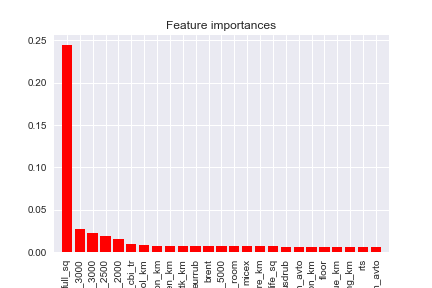
\includegraphics[width=15cm]{./output_images/importance.png}
\caption{Feature importance}
\label{fig:thirteen}
\end{center}
\end{figure}

This makes sense, since one would expect that the most important features, with regard to sales price, would be the size of the property and recreational/entertainment features nearby (cafes, sports, etc...).

\section{Methodology}

As a starting point, \href{https://www.kaggle.com/bguberfain/naive-xgb-lb-0-317}{this} was used as a reference.

\subsection*{Data Preprocessing and Algorithm Implementation}
\indent \par There are a few different features that are not modeled as of yet, but could be important.  Such features include the month, day-of-week, and the year of the transaction.  It would seem reasonable that some months would be better for purchasing property than others; real estate may be less desirable in winter months, for example.  Also, the year of the transaction may be significant if there are significant economic or social trends that were important that year (e.g. the fall of the Soviet Union in the early-1990's).

\par The ratio of room space to total space may also be interesting.  For instance, someone might not want a tiny kitchen in an otherwise large home.  Also, apartments on the higher floors will most likely fetch higher prices than those on lower floors.  Therefore, one should look at the ratio of the floor to the maximum number of floors in an apartment building.  A small ``fudge-factor" is added to the division in the \textbf{rel\_floor} value computation to avoid divide-by-zero issues.

\par It should be clear from the heatmaps that the data is very \href{https://www.kaggle.com/robertoruiz/dealing-with-multicollinearity}{collinear}.  This would seem to indicate that there might be a gain in model performance if the feature set was reduced to a combination of linearly independent pseudofeatures.  This could be accomplished via \href{http://setosa.io/ev/principal-component-analysis/}{principal components analysis}.  First, a baseline needs to be established to see if PCA might help.  The $R^2$ score for the \textbf{XGBoost} baseline is 0.40971, with a public score of 0.39276.  Both of these scores are an improvement over those obtained using the benchmark.  In order to consider using PCA, there would need to be an improvement in $R^2$ score, the public score can be checked as an additional sanity measure.

\begin{center}
\captionof{table}{$R^2$ score vs. number of principal components- no whitening}
\begin{tabular}{c | c }
\hline
\# PC's & $R^2$ \\ \hline
 19 & 0.153 \\ \hline
57 & 0.180 \\ \hline
127 & 0.375 \\ \hline
182 & 0.374 \\ \hline
202 & 0.375 \\ \hline
205 & 0.374 \\ \hline
221 & 0.372 \\ \hline
261 & 0.376 \\ \hline
333 & 0.375 \\ \hline
369 & 0.374 \\ \hline
\end{tabular}
\label{tbl:two}
\end{center}

\par PCA didn't improve model performance (see Table \ref{tbl:two}).  In fact, performance was degraded.  It's clear that there seems to be nearly indistinguishable scores once the number of principal components exceeds some threshold (about 127 in this case).  There is another PCA option that can be utilized to try that might improve performance:  whitening.  Whitening the data is a way to further remove correlation from feature vectors resulting from a principal components transformation.

\begin{center}
\captionof{table}{$R^2$ score vs. number of principal components- whitening}
\begin{tabular}{c | c }
\hline
\# PC's & $R^2$ \\ \hline
 19 & 0.157 \\ \hline
57 & 0.182 \\ \hline
127 & 0.375 \\ \hline
182 & 0.373 \\ \hline
202 & 0.373 \\ \hline
205 & 0.373 \\ \hline
221 & 0.372 \\ \hline
261 & 0.374 \\ \hline
333 & 0.375 \\ \hline
369 & 0.374 \\ \hline
\end{tabular}
\label{tbl:three}
\end{center}

\par The results are indistinguishable from the non-whitening results (see Table \ref{tbl:three}).  Therefore it is concluded that it is not worth using principal components; stick with the dataset as-is and focus on tuning the hyperparameters for \textbf{XGBoost}.

\subsection*{Refinement}
\indent \par Following \href{https://www.analyticsvidhya.com/blog/2016/03/complete-guide-parameter-tuning-xgboost-with-codes-python/}{this procedure}, the tuning process is as follows:

\begin{center}
\captionof{table}{Tuning Process}
\begin{tabular}{c | c }
\hline
Step \# & Process \\ \hline
 1 & Tune \textbf{max\_depth} and \textbf{min\_child\_weight} \\ \hline
 2 & Tune \textbf{gamma} \\ \hline
 3 & Tune \textbf{subsample} and \textbf{colsample\_bytree} \\ \hline
 4 & Tune regularization parameters \\ \hline
 5 & Tune \textbf{learning\_rate} \\ \hline
 6 & Tune \textbf{n\_estimators} \\ \hline
\end{tabular}
\end{center}

The functions \textbf{RandomizedSearchCV} and \textbf{GridSearchCV} functions from \\\textbf{sklearn.model\_selection} are used for the optimization.  The resource referenced also provides the range of values to use for the tuning.  See \href{http://xgboost.readthedocs.io/en/latest/parameter.html}{this} for more details on hyperparameter descriptions.

\subsubsection*{Step 1:  Tune \textbf{max\_depth} and \textbf{min\_child\_weight}}

\indent \par The parameters \textbf{max\_depth} and \textbf{min\_child\_weight} are the number of layers of decision trees used and the minimum sum of instance weight in a tree's child, respectively.  The public score is 0.34795, which is a significant improvement over the previous score of 0.39276. The $R^2$ score is 0.41821.

\subsubsection*{Step 2:  Tune \textbf{gamma}}

\indent \par The hyperparameter \textbf{gamma} is the minimum loss reduction required to create a further partition.  This can also be thought of as information gain required from a certain split in order to make that split.

\par The public score for this step is 0.34814.  The best $R^2$ score is 0.41756.  Both the public and $R^2$ scores are not significantly different than those from the previous step.  Both are still an improvement over the random forest baseline.

\subsubsection*{Step 3:  Tune \textbf{subsample} and \textbf{colsample\_bytree}}

\indent \par The hyperparameters \textbf{subsample} and \textbf{colsample\_bytree} are the subsample ratio of training data and the subsample ratio of columns when constructing a new tree, respectively.  The first parameter is to prevent overfitting to the training data.

\par The public score for this step is 0.34924.  The best $R^2$ score is 0.41667.  Both the public and $R^2$ scores are not significantly different than those from the previous step.  Both are still an improvement over the random forest baseline.

\subsubsection*{Step 4:  Tune regularization parameters}
\indent \par The hyperparameters \textbf{reg\_alpha} and \textbf{reg\_lambda} are the \href{http://cs.nyu.edu/~rostami/presentations/L1_vs_L2.pdf}{L1 and L2 regularization terms}, respectively. The function \textbf{GridSearchCV} is used due to the scale desired on the L1 term \textbf{reg\_alpha}. It would be difficult to randomly sample and hit the desired scales to test for this hyperparameter.

\par The public score for this step is 0.35830.  The $R^2$ score is 0.41689.  The public score degradation is a more significant difference than those observed in previous steps, and therefore this step is not implemented in the final solution.

\subsubsection*{Step 5:  Tune \textbf{learning\_rate}}
\indent \par One potential \href{http://machinelearningmastery.com/tune-learning-rate-for-gradient-boosting-with-xgboost-in-python/}{issue} with \textbf{XGBoost}, and boosting algorithms in general, is that the model can learn too quickly and overfit to the training data.  Therefore, it is desirable to slow the learners and prevent this overfitting.  The hyperparameter \textbf{learning\_rate} (though it is called \textbf{eta} in the \textbf{XGBoost} package) represents this learning rate.

\par The public score is 0.33300 and the $R^2$ score is 0.42211.  This is an improvement in both public and $R^2$ scores!  In fact, this is better than any step so far, which is the ultimate goal.

\subsubsection*{Step 6:  Tune \textbf{n\_estimators}}
\indent \par The hyperparameter \textbf{n\_estimators} is the number of trees to fit.  The \textbf{GridSearchCV} function is used here due to the scale desired to test.

\par The optimal number of estimators appears to be 500, as we've been using all along.  Since the results of this step are equivalent to those of Step 5, the public score is not reported.

\section{Results}

\subsection*{Model Evaluation and Validation}
\indent \par The process outlined above for arriving at a final model is reasonable; model hyperparameters were chosen at each step that improve $R^2$ and public leaderboard scores over a benchmark model.  However, a single validation set was used in the tuning.  Now, it is necessary to test for generalization to unseen data; that is, using multiple training and validation sets and comparing model performance across these multiple sets.  This can be done using \href{http://scikit-learn.org/stable/modules/cross_validation.html}{cross-validation} (\href{https://www.analyticsvidhya.com/blog/2016/01/complete-tutorial-learn-data-science-python-scratch-2/}{here} is another useful link).  The package \textbf{sklearn.model\_selection} has two utilities that will be needed to do this analysis: \textbf{learning\_curve} and \textbf{ShuffleSplit}.  The function \textbf{learning\_curve} computes $R^2$ scores for training and validation scores across a cross-validation generator.  The function \textbf{ShuffleSplit} creates cross-validation datasets based upon the desired number of instances, train-validation split ratio, and a random seed.  The training and cross-validation scores for the regressor tuned in the last section are shown in Figure \ref{fig:fourteen}.

\begin{figure}[h!]
\begin{center}
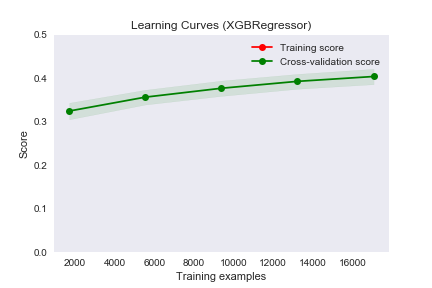
\includegraphics[width=12cm]{./output_images/xgb_cv.png}
\caption{Cross validation- tuned XGBoost}
\label{fig:fourteen}
\end{center}
\end{figure}

The two mean scores lie directly on top of one another, indicating that the performance on the training and validation sets matches very closely, nearly perfectly, in fact.  Any error would be well-within the 1-sigma uncertainty bounds, indicated by the green solid area bisected by the mean scores.  It can be concluded that the model generalizes very well to unseen data.  The data appear to be approaching an asymptote, however this asymptote appears to be less than 0.5 even, indicating that housing price is not fully predictable given the feature set used.  The plot also indicates that performance could be improved with more training examples.

\subsection*{Justification}

To justify the use of this model, a simple comparison to the benchmark can be made.  A good place to start would be to repeat the above cross-validation on the benchmark model.

\begin{figure}[h!]
\begin{center}
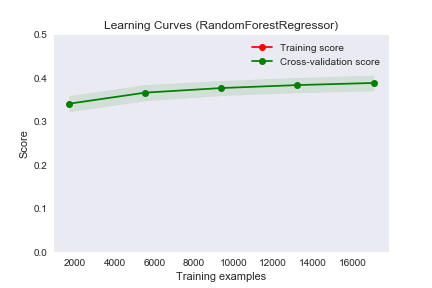
\includegraphics[width=12cm]{./output_images/rgr_cv.png}
\caption{Cross validation- Random Forest}
\label{fig:fifteen}
\end{center}
\end{figure}

Figure \ref{fig:fifteen} shows subtle differences from the cross-validation plot for the tuned regressor.  First, there are some similarities.  Most notably, this regressor would perform better with more training results.  The asymptotic value that the data appears to be approaching is lower than that of the tuned regressor plot; the slope of the mean score line is flatter in this plot.  It appears as though maximum value of the $R^2$ score for this regressor will occur for a smaller training sample size than the maximum obtained for the tuned regressor.  As in the tuned regressor case, the model generalizes well to unseen data.

The final solution is significant enough to solve the problem at hand.  The model gives reasonable performance given the complexity of the data and the minimal addition of features extracted from the raw data.  Practically, there is only so much training data that is available.  If more data were available, the model performance would be a little better, but nowhere near 1, as indicated by the cross-validation plot.  This solution is favorable over more complex solutions (such as stacked regressors) since it is easy to implement, easy to interpret, and provides adequate performance.

\section{Conclusion}

\subsection*{Free-Form Visualization}
\indent \par There is one table that hasn't been shown yet, but summarizes the analysis quite well.

\begin{center}
\captionof{table}{Performance summary}
\begin{tabular}{c | c | c | c | c}
\hline
Regressor & $R^2$ score & Improvement & Kaggle Public Score & Improvement \\ \hline
Random Forest & 0.39009 & N/A &  0.41668 & N/A \\ \hline
XGBoost Baseline & 0.40971 & +0.050 &  0.39276 & -0.046 \\ \hline
XGBoost Step 1 & 0.41860 & +0.069 &  0.34795 & -0.155 \\ \hline
XGBoost Step 2 & 0.41756 & +0.071 &  0.34814 & -0.154 \\ \hline
XGBoost Step 3 & 0.41667 & +0.068 &  0.34924 & -0.152 \\ \hline
XGBoost Step 4 & 0.41689 & +0.069 &  0.35830 & -0.130 \\ \hline
XGBoost Step 5 & 0.42211 & +0.082 &  0.33300 & -0.191 \\ \hline
XGBoost Step 6 & 0.42211 & +0.082 &  0.33300 & -0.191 \\ \hline
\end{tabular}
\label{tbl:four}
\end{center}

Table \ref{tbl:four} shows improvement of each step over the benchmark.  The \textbf{Improvement} columns show the results of the relative improvement over the benchmark, computed as 
\beq
\text{Improvement} = \frac{s_{\text{step}} - s_{\text{benchmark}}}{s_{\text{benchmark}}}, 
\eeq
where $s_*$ denotes a particular score, either $R^2$ or the Kaggle public score.  These columns can be interpreted, after multiplying by 100, as the percent relative change in the scores from the benchmark compared to each step.  The sought after trends are a positive change in $R^2$ score and a negative change in the Kaggle public score.  The table shows that, through tuning, an 8\% positive change in $R^2$ score, along with a large 19\% relative change in public score, were achieved.

\subsection*{Reflection}
\indent \par A model was developed for predicting the sales price of properties within the Russian housing market based upon features provided by Sberbank, a Russian bank.  Plots were presented, and analyzed, showing trends in both micro- and macroeconomic features, and the relationship of these features to sales price.  Minimal feature engineering was performed on the dataset to provide a few additional, potentially important features.  A benchmark model based on an untuned random forest regressor was presented as an initial first cut at a solution.  Based upon previous analyses and their results, \textbf{XGBoost} was selected, and tuned, as the final solution for this problem.  \textbf{XGBoost} provided a nice framework to build upon since it requires minimal feature engineering and scaling to achieve best results.

Quite surprising was the fact that PCA didn't really improve performance, despite the high degree of multicollinearity observed in the data.  Perhaps naively, one would think that creating a new pseudofeature set that orthogonally spans the feature space would allow for greater predictive power of the underlying model.  However, the results seem to confirm the previous notion that decision trees are \href{https://stats.stackexchange.com/questions/141864/how-can-top-principal-components-retain-the-predictive-power-on-a-dependent-vari}{insensitive to principal component reduction}.

This project presented some difficulties in interpreting the data provided.  There were many features, and many of these features seemed very interrelated.  There was also much data missing.  Fortunately, there are good standalone packages within \textbf{sklearn} for dealing with such cases.  In the end, it was great that there exists a simple-to-use framework, \textbf{XGBoost}, that made working with the data very easy.

The final model fits expectations, and the process followed for tuning was very straightforward.  A similar process could be used for solving problems of a similar type: data analysis, data reduction/scaling, feature engineering, and regressor development are the common steps for any regression analysis.  Depending upon the data involved, it may not be necessary to use as strong a learner as \textbf{XGBoost}; a simple linear regressor may be adequate if the degree of nonlinearity in the target variable is low.  Given the data observed in the cross-validation plots and the amount of training data available, it seems that this model performs about as well as can be expected for a single regressor approach.

\subsection*{Improvement}
\indent \par It would seem that better performance might be achieved if multiple learners were combined.  Some algorithms may achieve better performance for some regions in the feature space while others might perform better elsewhere.  The package \href{https://github.com/rasbt/mlxtend}{\textbf{mlxtend}} provides a \textbf{Python} framework for doing stacked regression.  Stacked regression provides a way of combining multiple regressors into a single predictor, and has been shown to \href{http://blog.kaggle.com/2016/12/27/a-kagglers-guide-to-model-stacking-in-practice/}{work well in other Kaggle competitions}.  There is a trade-off here, though.  Typically, the added complexity comes with relatively modest improvements.  This added complexity may obscure any interpretation of the model; functional relationships between features and target variables may be more difficult to establish despite any observed increases in predictive power (i.e. $R^2$ score).

%%\begin{figure}[h!]
%%\begin{center}
%%\includegraphics[width=8cm]{efstab.jpg}
%%\caption{Explicit Euler stability properties}
%%\end{center}
%%\end{figure}
%%\subsubsection*{Implicit Euler}
%%\beq
%%p(h) &=& \frac{1}{1+h} \\
%%\implies 0 &<& h < \infty \text{ is the region of stability}
%%\eeq
%%\begin{figure}[h!]
%%\includegraphics[width=8cm]{cp1.jpg}
%%\includegraphics[width=8cm]{cp01.jpg}
%%\caption{Left: $h = 0.1$ and Right: $h = 0.01$}
%%\end{figure}
\end{document}